Inspired by nature, engineers are moving away from rigid robotics, and towards compliant, soft robotics.
In particular, the focus is on exoskeleton gloves which wrap around the user's hand, and aim to support basic functions -- such as grasping and pinching, which may have been partially or totally lost.
The exact combination of material and actuation varies wildly, but the one of interest is made out of an elastomer -- that is, an elastic polymer; and it is activated by a button, which in turn move metal wires that mimic tendons.
Figure \ref{fig:Wearable_Glove} is a representation of what it looks like.

\begin{figure}[h]
    \centering
    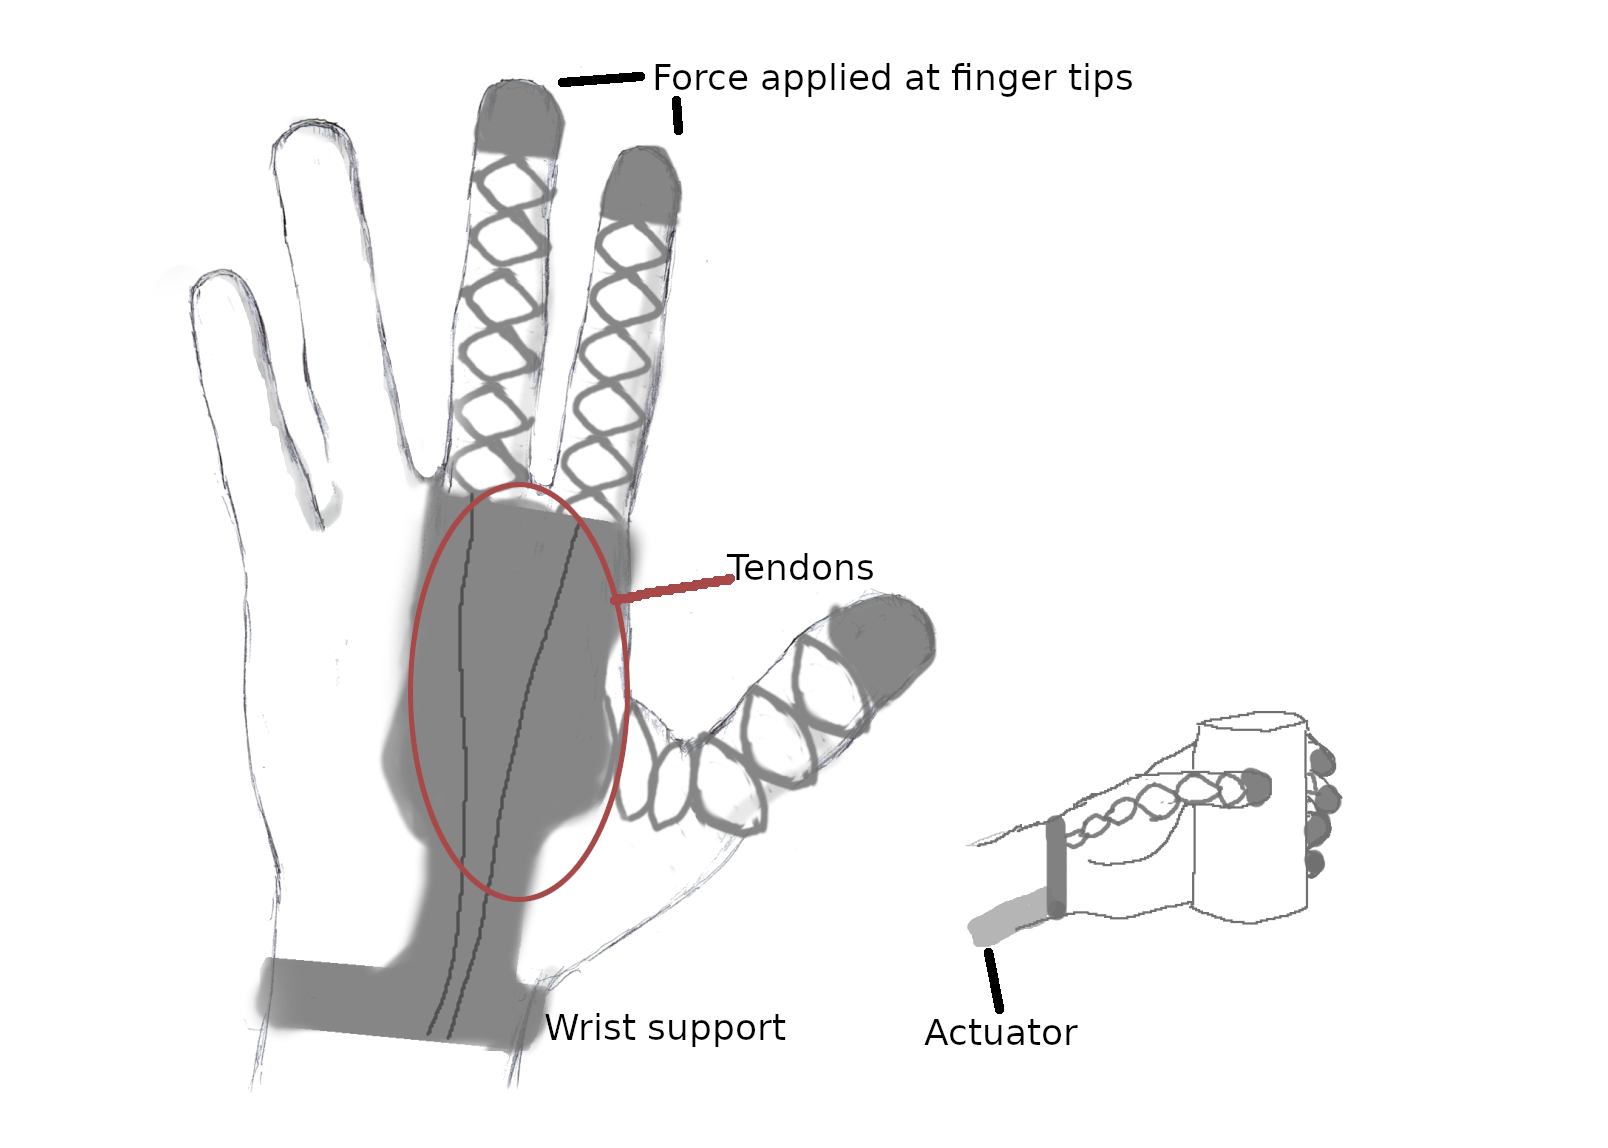
\includegraphics[width=0.8\columnwidth]{files/Gloves.png}
    \caption{Wearable soft robot based on In's 2011 design \citep{InHyunki2011Jsau}. }
    \label{fig:Wearable_Glove}
\end{figure}

Wearable soft robots present a very interesting tool to increase the level of independence experienced by a person with loss of manual motor skills.
One area that presents an interesting ethical issue is that this product is targeted towards a very specific group, which does not presently have commercially widespread alternative solutions.
In effect this presents a captive market, where manufacturers may have the opportunity to charge the customers far more than is reasonable.

Furthermore, alternatives currently in development may focus on individual finger motion and occupational therapy \citep{CianchettiMatteo2018Baos,ConnellyLauri2010APGa}, while Exo-Glove Poly -- our glove in question -- is merely to support gross motions.
This is an important ethical concern -- that of not misleading consumers. The aim of this product is not therapeutic, and there are alternatives being designed and tested for that purpose in particular.
Its use may not be detrimental to one who requires the therapeutic product, but one should not knowingly mislead one's target audience.

Finally, it is vital that a product such as this is only made available to the public when it is deemed safe.
Consider that its aim is to provide more independence to those who often will have a supporting party with them.
A failure in the mechanisms may put them not only in direct danger, but also if the person is unaccompanied, it may escalate the amount of danger, as they may not be able to immediately seek help.

In conclusion, products targeted at particularly vulnerable groups require very high ethical standards -- even when their aim is purely supportive.